17. Построим по двум точкам $(0;-3)$ и $\left(\cfrac{3}{4};0
ight)$ график функции $y=4x-3$ и отразим его вверх симметрично относительно оси абсцисс.
$$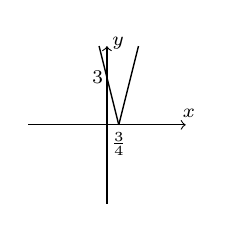
\begin{tikzpicture}[scale=0.2]
\tikzset {line01/.style={line width =0.5pt}}
\tikzset{line02/.style={line width =1pt}}
\tikzset{line03/.style={dashed,line width =0.5pt}}
%\filldraw [black] (0,0) circle (1pt);
\draw [->] (-5,0) -- (5,0);
\draw [->] (0,-5) -- (0,5);
\draw[line01] (0.75,0) -- (2,5);
\draw[line01] (0.75,0) -- (-0.5,5);
\draw (5.2,0.7) node {\scriptsize $x$};
\draw (-0.6,3) node {\scriptsize $3$};
\draw (0.75,-1.2) node {\scriptsize $\frac{3}{4}$};
\draw (0.7,5.2) node {\scriptsize $y$};
\end{tikzpicture}$$
